\nTitle{Programmation Linéaire monocritère}

\section{Données}
Soient :
\begin{itemize}
  \item \textbf{T} la matrice des temps unitaires d'usinage d'un produit sur une
  machine (minutes) (\textsl{C.f. Table 1}).
  \item \textbf{Q} la matrice de quantité de matières premières par produit
  (\textsl{C.f. Table 2}).
  \item \textbf{S} la matrice des quantité maximum de matières premières
  (\textsl{C.f. Table 3}).
  \item \textbf{V} la matrice des prix de vente des produits finis (\textsl{C.f.
  Table 4})
  \item \textbf{A} la matrice des prix d'achat des matières premières.
  \item \textbf{C} la matrice des coûts horaires des machines (\textsl{C.f.
  Table 5}).
\end{itemize}
 
\subsection{Contraintes}
Considérons :
\begin{itemize}
  \item 6 produits identifiés chacun par une lettre $i \in {A, B, C, D, E, F}$
  \item 7 machines identifiée chacune par un nombre $j \in {1, 2, 3, 4, 5, 6 ,7}$
  \item 3 matières premières identifiée chacune par un nombre $k \in {1, 2, 3}$
  \item $n$, vecteur colonne du nombre d'unités fabriquées pour chaque produit
\end{itemize}
~\\
L'ensemble de la chaine de production est régie par les contraintes suivantes
:\\
\begin{itemize}
  \item \textbf{Le nombre de produits usinés de type $i$ :} Il doit être non nul
  \begin{equation} 
  	n_i \ge 0, \forall i \in {A, B, C, D, E, F} \label{C0}
  \end{equation}
  
  \item \textbf{Le temps d'occupation de chaque machine $i$:} Il doit être
  inférieur au temps de travail
  \begin{equation} 
  	\sum_{j = A}^{F} T_{j,i} \times n_j \leq 2 \times 8 \times 60 \times 5 = 4800, \forall i \in {1, 2, 3, 4, 5, 6 ,7} \label{C1}
  \end{equation} 
  soit un temps de travail en deux huit, 5 jours par semaine.
  
  \item \textbf{L'utilisation de chaque matière première  $i$:} Elle doit être
  inférieure au stock
  \begin{equation} 
  	\sum_{j = A}^{F} Q_{i,j} \times n_j \leq S_i, \forall i \in {1,2,3} \label{C2}
  \end{equation} 
\end{itemize}

\newpage
\subsubsection{Modélisation sous forme matricielle}
Pour donner au problème une forme standard, nous allons le modéliser par des inéquations et des produits matriciels.
Les contraintes C0, C1 et C2 se traduisent trivialement de la manière suivante :

\begin{equation}
A.n \leq b
\end{equation}
Avec :
\[
A =
\begin{pmatrix}
\\
\\
\quad & \quad & -I & \quad & \quad \\
\\
\\
\\
\hline
\\
\\
\\
\quad & \quad & T^{t} & \quad & \quad \\
\\
\\
\\
\hline
\\
\quad & \quad & Q & \quad & \quad \\
\\
\end{pmatrix}
, b = 
\begin{pmatrix}
0 \\ 0 \\ 0 \\ 0 \\ 0 \\ 0 \\
\hline
4800 \\ 4800 \\ 4800 \\ 4800 \\ 4800 \\ 4800 \\ 4800 \\
\hline
\\
S^{t} \\
\\
\end{pmatrix}
\]

Ce qui nous donne plus concrètement les matrices suivantes :
\[
A =
\begin{pmatrix}
   -1 &    0 &    0 &    0 &    0 &    0 \\
    0 &   -1 &    0 &    0 &    0 &    0 \\
    0 &    0 &   -1 &    0 &    0 &    0 \\
    0 &    0 &    0 &   -1 &    0 &    0 \\
    0 &    0 &    0 &    0 &   -1 &    0 \\
    0 &    0 &    0 &    0 &    0 &   -1 \\
\hline
    8 &   15 &    0 &    5 &    0 &   10 \\
    0 &    1 &    2 &   15 &    7 &   12 \\
    8 &    1 &   11 &    0 &   10 &   25 \\
    2 &   10 &    5 &    4 &   13 &    7 \\
    5 &    0 &    0 &    0 &   10 &   25 \\
    5 &    5 &    3 &   12 &    8 &    0 \\
    5 &    3 &    5 &    8 &    0 &    0 \\
\hline
    1 &    2 &    1 &    5 &    0 &    2 \\
    2 &    2 &    1 &    0 &    2 &    1 \\
    1 &    0 &    3 &    2 &    2 &    0 \\
\end{pmatrix}
, b = 
\begin{pmatrix}
0 \\ 0 \\ 0 \\ 0 \\ 0 \\ 0 \\
\hline
4800 \\ 4800 \\ 4800 \\ 4800 \\ 4800 \\ 4800 \\ 4800 \\
\hline
350 \\ 620 \\ 485
\end{pmatrix}
\]

\section{Objectif : Comptable}
Le comptable cherche à maximiser les bénefices sous les contraintes définies
précedemment.

\subsection{Modélisation}
Soit $n_i$ le nombre de produit $i$ fabriqué. Le coup fixe de production
n'influant pas sur notre décision, nous ne considérerons que le coût variable de
production. Il est défini par la formule suivante:
\begin{displaymath}
CV(i) = n_i * \left (\sum_{j = 1}^{7} T_{i,j} .
\frac{C_{i,j}}{60} + \sum_{k = 1}^{3} Q_{k,i} . A_{k} \right )
\end{displaymath}
~\\
Le chiffre d'affaire par produit est :
\begin{displaymath}
CA(i) = n_i . V_i
\end{displaymath}
~\\
Par conséquent le bénefice par produit se calcule de la manière suivante :
\begin{eqnarray*}
	B(i) &=& CA(i) - CV(i)\\
	B(i) &=& n_i * \left (V_i - \sum_{j = 1}^{7} T_{i,j} . \frac{C_{i,j}}{60} +
	\sum_{k = 1}^{3} Q_{k,i} . A_{k} \right )
\end{eqnarray*}
\newpage
\section{Objectif : Responsable d'atelier}
Le responsable d'atelier cherche à maximiser le nombre d'unités (toutes
catégories confondues) produites sous les contraintes définies précedemment.

\subsection{Modélisation}
Soit $N$ le nombre de produits fabriqués.

\begin{equation}
	N = \sum_{i = A}^{F}
\end{equation} 
\newpage
\section{Objectif : Responsable commercial}
Le responsable commercial cherche à équilibrer le nombre
d'unités de ${A, B, C}$ (famille 1) et ${D, E, F}$ (famille 2) afin que ces deux
familles contiennent le même nombre d'unités ( à $\epsilon$
unité(s) près).\\
Autrement dit, l'écart entre le nombre d'unités produite pour la famille A et la famille B doit être inférieur à un seuil $\epsilon$.

\subsection{Modélisation}
Soient :
\begin{itemize}
  \item $N_1$ le nombre de produits de la famille 1 fabriqués.
  \item $N_2$ le nombre de produits de la famille 2 fabriqués.
\end{itemize}

\begin{eqnarray*}
	|N_1 - N_2| &\leq& \epsilon\\
	\Leftrightarrow -\epsilon \leq N_1 - N_2 &\leq& \epsilon\\
	\Leftrightarrow -\epsilon \leq \sum_{i = A}^{C} n_i - \sum_{j = D}^{F} n_j
	&\leq& \epsilon\\
\end{eqnarray*} 
Par concéquent, c'est cette nouvelle contrainte qui, venant s'ajouter aux
contraintes précédentes, va permettre de calculer le nombre d'unités A, B, C,
D, E, et F à fabriquer afin d'équilibrer les deux familles.\\
~\\
Nous obtenons la matrice suivante :
\begin{displaymath}
M = \left(
\begin{array}{cccccc}
1 & 1 & 1 & 1 & 1 & 1\\
\end{array}
\right)
\end{displaymath}
La matrice, très simple, représente la somme des différents produits.\\
La matrice des contraintes devient quant à elle :
INSÉRER MATRICE A MODIFIEE

\subsection{Décisions}

\subsection{Interprétation}
Evidemment, toutes les solutions triviales du type :
\begin{displaymath}
M_p = \left(
\begin{array}{cccccc}
N \pm \epsilon & N \pm \epsilon & N \pm \epsilon & N & N & N\\
\end{array}
\right)
\end{displaymath}
ou encore 
\begin{displaymath}
M_p = \left(
\begin{array}{cccccc}
N & N & N & N \pm \epsilon & N \pm \epsilon & N \pm \epsilon\\
\end{array}
\right)
\end{displaymath}
\begin{center}
\textsl{Où $M_p$ est la matrice du nombre de produit, et $N \in \mathbbm{N}$}
\end{center}
sont des solutions \emph{valables}.\\
~\\
Ceci met en évidence qu'avec les critères définis plus haut, il n'y a pas de
solution plus \og valable\fg ~qu'une autre. Par concéquent nous pouvons :
\begin{itemize}
  \item Choisir une solution au hasard
  \item Augmenter le nombre de critère et notamment ceux en rapport avec les
  stocks disponibles, le prix des matières premières, ou encore le temps
  d'usinage nécessaire.
\end{itemize}

\newpage
\section{Stratégie du point de vue du \textsl{Responsable des stocks}}
\label{sec:stocks}

Le responsable des stocks cherche à minimiser la contenance du stock,
\textsl{i.e.} le nombre de produits entreposés ajouté à la quantité de
matières premières. Aucune contrainte particulière n'est ajoutée mais la
recherche de l'optimum se fait sous les contraintes définies précédemment.

\subsection{Modélisation}
Soit $Stock(n_{i})$ le nombre d'unités de stock nécessaires pour stocker les
produits fabriqués et les matières premières nécessaires.\\
Cette fonction est évidemment la somme des produits fabriqués et de la quantité de matières
premières nécessaire à leur fabrication.\\
~\\
Supposons qu'\textbf{un produit fabriqué correspond à une unité de stock.}\\
~\\
Ainsi, soient :
\begin{itemize}
	\item $n_{i}$ la quantité de produits usinés (pour chaque produit $i$)
	\item $Q_{j,i}$ la quantité de matière première par produit pour chaque produit $i$ et chaque matière première $j$.
\end{itemize}
~\\
Alors :
\begin{equation}
	Stock(n) = \sum_{i} (n_{i} + n_{i} \times \sum_{j} Q_{j,i})
\end{equation}

La représentation matricielle de cette fonction sera alors :

\begin{equation}
	M_S = \begin{pmatrix}
		1 & 1 & 1 & 1 & 1 & 1
	\end{pmatrix} + (
	\begin{pmatrix}
		1 & 1 & 1
	\end{pmatrix}
	\times Q)
\end{equation}

\subsection{Stratégie adoptée}
Un résultat trivial est de ne fabriquer aucun produit :
\begin{equation}
    \begin{pmatrix}
	0 \\ 0 \\ 0 \\ 0 \\ 0 \\ 0
    \end{pmatrix}
\end{equation}

En effet, en l'absence de production, aucun stock n'est nécessaire. Ce résultat
n'est pas satisfaisant.\\
Nous allons donc nous intéresser à un second critère : \textbf{les bénéfices de l'entreprise}.\\
Pour ce faire, nous allons nous utiliser les résultats obtenus en imposant un minimum de bénéfices.\\
En réalisant les calculs sur plusieurs échelons, nous obtenons un résultat linéaire par morceaux. Le
raisonnement adopté est similaire à celui développé dans la section \ref{sec:monocrit}.

\begin{figure}[!ht]
	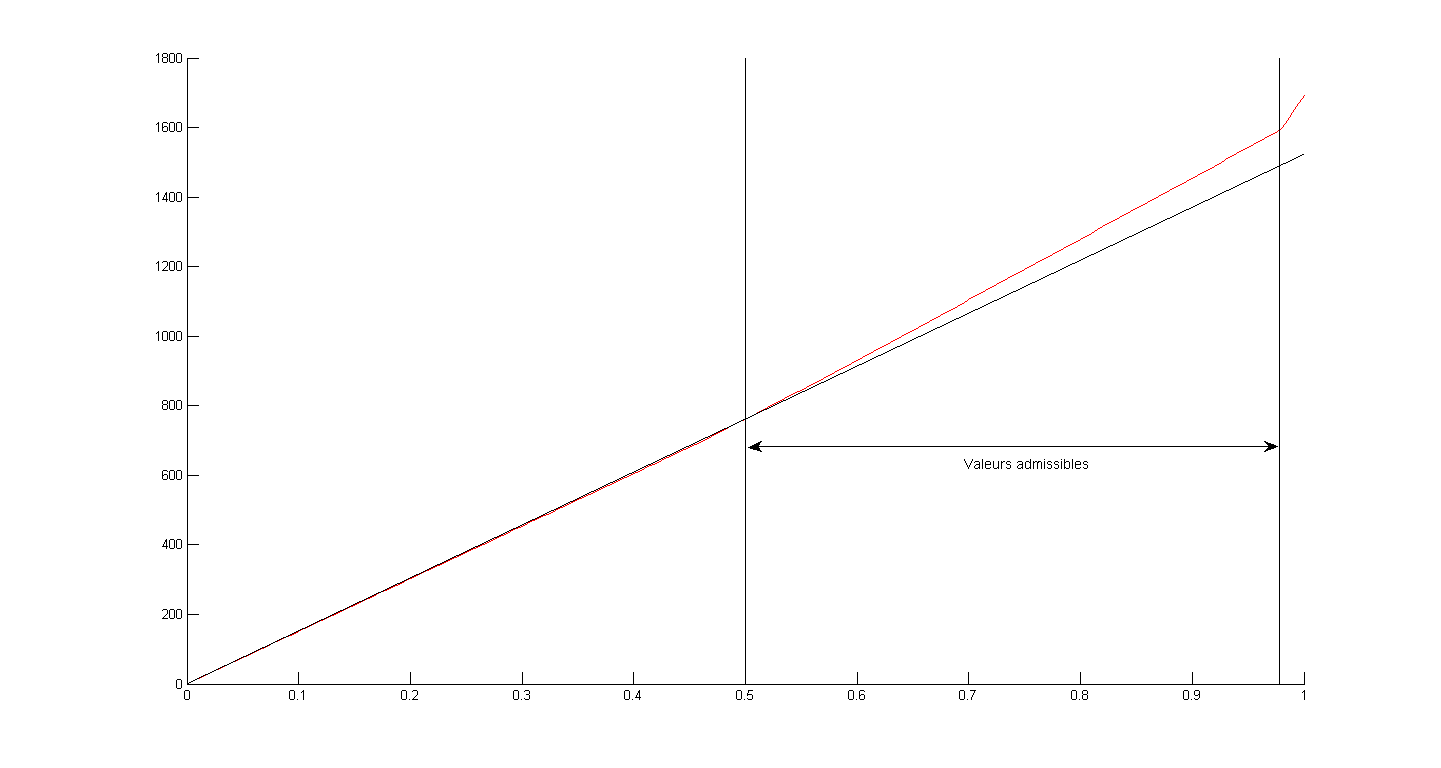
\includegraphics[width=\textwidth]{graphe_resp_stocks.png}
	\caption{Graphe de l'évolution des stocks en fonction du bénéfice}
\end{figure}

\subsubsection{Interprétation} 
De nombreuses valeurs sont équivalentes mathématiquement parlant et ne peuvent pas vraiment être départagées. 
Les choix possibles se situent dans la deuxième partie de la courbe :
\begin{itemize}
	\item En dessous, les bénéfices sont trop bas.
	\item Au dessus, les besoins de stockage augmentent beaucoup plus que les bénéfices. Nous perdons alors de vu notre
	objectif initial, \textsl{i.e.} avoir le moins de stock possible.
\end{itemize}

Nous obtenons donc une valeur comprise entre 50\% et 98\% de bénéfices. 
Pour 75\% du bénéfice maximum, nous obtenons le nombre de produits suivants :

\begin{equation}
\begin{pmatrix}
1,91903382074088 \times 10^{-10} \\
2,63753463514149 \times 10^{-10} \\ 
1,89174897968769 \times 10^{-10} \\
1,23691279441118 \times 10^{-10} \\ 
124,634235411818 \\
142,146305832495 
\end{pmatrix}
\end{equation}

\begin{center}
	\fbox{\textbf{Soit une quantité d'unités en stock de 1191,75640039347.}}
\end{center}
~\\
Cette étude de cas nous rappelle les limite d'une stratégie basée sur l'analyse d'un seul critère. En effet, 
en l'absence de contraintes assez fortes, le problème devient \og indécidable\fg mathématiquement.

C'est pourquoi nous allons combiner les 4 études réalisées pour affiner nos stratégies et obtenir une solution : 
\begin{itemize}
	\item Mathématiquement claire
	\item Respectant un ensemble de contraintes plus grand, et par conséquent qui se concentre plus sur les
	contraintes propres à l'entreprise \textbf{Optim}.
\end{itemize}

